%%%%%%%%%%%%%%%%%%%%%%%%%%%%%%%%%%%%%%%%%%%%%%%%%%%%%%%%%%%%%%%%%%%%%%%%%%%%%%%%%%%%%%%%%%%%%%%%%%%%%%%%%%%%%%%%%%%%%%%%%%%%%%%%%%%%%%%%%%%%%%%%%%%%%%%%%%%%%%%%%%%
% Written By Michael Brodskiy
% Class: Fundamentals of Electromagnetics
% Professor: E. Marengo Fuentes
%%%%%%%%%%%%%%%%%%%%%%%%%%%%%%%%%%%%%%%%%%%%%%%%%%%%%%%%%%%%%%%%%%%%%%%%%%%%%%%%%%%%%%%%%%%%%%%%%%%%%%%%%%%%%%%%%%%%%%%%%%%%%%%%%%%%%%%%%%%%%%%%%%%%%%%%%%%%%%%%%%%

\documentclass[12pt]{article} 
\usepackage{alphalph}
\usepackage[utf8]{inputenc}
\usepackage[russian,english]{babel}
\usepackage{titling}
\usepackage{amsmath}
\usepackage{graphicx}
\usepackage{enumitem}
\usepackage{amssymb}
\usepackage[super]{nth}
\usepackage{everysel}
\usepackage{ragged2e}
\usepackage{geometry}
\usepackage{multicol}
\usepackage{fancyhdr}
\usepackage{cancel}
\usepackage{siunitx}
\usepackage{physics}
\usepackage{tikz}
\usepackage{mathdots}
\usepackage{yhmath}
\usepackage{cancel}
\usepackage{color}
\usepackage{array}
\usepackage{multirow}
\usepackage{gensymb}
\usepackage{tabularx}
\usepackage{extarrows}
\usepackage{booktabs}
\usepackage{lastpage}
\usepackage{float}
\usetikzlibrary{fadings}
\usetikzlibrary{patterns}
\usetikzlibrary{shadows.blur}
\usetikzlibrary{shapes}

\geometry{top=1.0in,bottom=1.0in,left=1.0in,right=1.0in}
\newcommand{\subtitle}[1]{%
  \posttitle{%
    \par\end{center}
    \begin{center}\large#1\end{center}
    \vskip0.5em}%

}
\usepackage{hyperref}
\hypersetup{
colorlinks=true,
linkcolor=blue,
filecolor=magenta,      
urlcolor=blue,
citecolor=blue,
}


\title{Exam 1}
\date{\today}
\author{Michael Brodskiy\\ \small Professor: E. Marengo Fuentes}

\begin{document}

\maketitle

\begin{enumerate}

  \item 

    \begin{enumerate}

      \item 

        The speed of wave propagation, $v_p$ can be defined as:

        $$v_p=\frac{c}{\sqrt{\varepsilon_o\mu_o}}$$

        Since we can assume the medium through which we are passing possesses no unusual magnetic properties, we can say $\mu_o=1$. Thus, we are left with:

        $$v_p=\frac{c}{\sqrt{\varepsilon_o}}$$

        This then gives:
        
        $$v_p=\frac{c}{\sqrt{2.25}}$$
        $$=\frac{3\cdot10^8}{2.25}$$
        $$\boxed{v_p=2\cdot10^8\left[ \frac{\si{\meter}}{\si{\second}} \right]}$$

      \item 

        The wavelength can be defined as the ratio of the speed of wave propagation to the frequency. This gives us:

        $$\lambda=\frac{v_p}{f}$$
        $$=\frac{2\cdot10^{8}}{1\cdot10^9}$$
        $$\boxed{\lambda=.2[\si{\meter}]}$$

      \item 

        The reflection coefficient may be defined as:

        $$\Gamma=\frac{z_L-z_o}{z_L+z_o}$$
        $$=\frac{(50-100j)-50}{(50-100j)+50}$$
        $$=\frac{-100j}{100-100j}\cdot\frac{100+100j}{100+100j}$$
        $$=\frac{-10000j+10000}{(100)^2-(100j)^2}$$
        $$=\frac{-10000j+10000}{20000}$$
        $$\boxed{\Gamma=.5-.5j}$$

        The reflection coefficient is unitless.

      \item 

        The standing wave ratio can be defined as:

        $$SWR=\frac{1+|\Gamma|}{1-|\Gamma|}$$

        where $|\Gamma|$ is the magnitude of the reflection coefficient. Thus, we get:

        $$|\Gamma|=\sqrt{.5^2+.5^2}=.7071$$
        $$SWR=\frac{1+.7071}{1-.7071}$$
        $$=\frac{1.7071}{.2929}$$
        $$\boxed{SWR=5.8284}$$

        The standing wave ratio is also unitless.

      \item 

        Since the function is written as cosine, we know:

        $$\left\{\begin{array}{l l}\text{Phase: } & -30^{\circ}\\\text{Magnitude: } & 10\end{array}$$

          Thus, we can write the phasor (in rectangular form) as:

          $$10\cos(-30^{\circ})+10\sin(-30^{\circ})j$$
          $$\boxed{\mathbb{V}_g=8.6603-5j}$$

          Alternatively, the phasor may be written as:

          $$\boxed{\mathbb{V}_g=10\angle-30^{\circ}\text{ or }10\angle-\frac{\pi}{6}}$$

      \item 

        We know the input impedance of a lossless medium is given by:

        $$z_{in}=z_o\left[ \frac{z_L+jz_o\tan(\beta l)}{z_o+jz_L\tan(\beta l)} \right]$$

        We can find $\beta$, since we know $\beta=\frac{2\pi}{\lambda}$:

        $$\beta=\frac{2\pi}{.2}=10\pi=31.415\left[ \frac{\text{rad}}{\si{\meter}} \right]$$

        Since we are trying to find the impedance at the start of the transmission line, we can use $l=.45[\si{\meter}]$:

        $$\tan(31.415*.45)=2398.4$$

        Now, we plug this into our equation to obtain the answer:

        $$z_{in}=50\left( \frac{50-100j+j(50)(2398.4)}{50+j(50-100j)(2398.4)} \right)$$
        $$\boxed{z_{in}=9.9967+19.9767j}$$

      \item 

        We can find the input voltage using:

        $$\mathbb{V}_{in}=\left( \frac{\mathbb{V}_gz_{in}}{z_g+z_{in}} \right)$$

        This gives us:

        $$\mathbb{V}_{in}=\left( \frac{(8.6603-5j)(9.9967+19.9767j)}{34.967+19.9767j} \right)$$
        $$\boxed{\mathbb{V}_{in}=5.5319 + 0.3575j}$$

      \item 

        We now need to convert from the phasor form of the voltage above to the time domain of the voltage. We begin by finding the magnitude:

        $$|\mathbb{V}_{in}|=\sqrt{5.5319^2+.3575^2}=5.5434$$

        We then find the angle:

        $$\theta=\tan^{-1}\left(\frac{.3575}{5.5319}\right)=.064535[\text{rad}]$$
        $$\theta=.064535[\text{rad}]\cdot\frac{360}{2\pi}=3.6976^{\circ}$$

        Putting these together, we get:

        $$\boxed{V_{in}(t)=5.5434\cos(\omega t+3.6976^{\circ})\text{ or }5.5434\cos(\omega t+.064535)}$$

      \item 

        We can find the voltage at any point using a similar formula to when we determined the input voltage:

        $$\mathbb{V}_0^+=\left( \frac{\mathbb{V}z_{in}}{z_g+z_{in}} \right)\left( \frac{1}{e^{14.137j}+(.5-.5j)e^{-14.137j}} \right)$$
        $$\mathbb{V}_0^+=-5.1751 - 5.8922j$$

        We must now incorporate an expression to account for the distance:

        $$\mathbb{V}=\mathbb{V}_0^+\left( e^{j\beta z}+\Gamma e^{-j\beta z} \right)$$
        $$=(-5.1751 - 5.8922j)\left( e^{j\beta z}+(.5-.5j)e^{-j\beta z} \right)$$
        $$=\left( (-5.1751 - 5.8922j)e^{j\beta z}+(-5.5336 - 0.3586j)e^{-j\beta z} \right)$$

        To simplify, we can convert so that the entire phasor is in exponential form:

        $$\mathbb{V}=7.8422e^{j(\beta z+48.707)}+5.5452e^{j(3.7078-\beta z)}$$

        We can then convert $\theta$ to radians for homogenous units (and shift by $\pi$ to make sure the values are negative when converted):

        $$\mathbb{V}=\underbrace{7.8422e^{j(10\pi z+(.8501-\pi))}}_{\text{incident wave}}+\underbrace{5.5452e^{j((0.064714-\pi)-10\pi z)}}_{\text{reflected wave}}$$
      $$\boxed{\mathbb{V}=\underbrace{7.8422e^{j(10\pi z-2.2915))}}_{\text{incident wave}}+\underbrace{5.5452e^{-j(3.0769+10\pi z)}}_{\text{reflected wave}}}$$

      \item 

        We can easily convert the phasor above to the time domain:

        $$\boxed{V(z,t)=\underbrace{7.8422\cos(\omega t+10\pi z-2.2915)}_{\text{incident wave}}+\underbrace{9.1569\cos(\omega t-10\pi z-3.0769)}_{\text{reflected wave}}}$$

      \item 

        The average power is given by the formula:

        $$P_L=(1-|\Gamma|^2)\frac{|V_0^+|^2}{2z_o}$$
        $$=(1-.5)\frac{7.8422^2}{2(50)}$$
        $$=(.5)\frac{7.8422^2}{2(50)}$$
        $$\boxed{P_L=.3075[\si{\watt}]}$$

    \end{enumerate}

  \item

    \begin{enumerate}
        
      \item 

        First and foremost, we must find the load impedance (marked by red dot in Figure \ref{fig:1}:

          $$Z_L=\frac{z_l}{z_o}=1-2j[\si{\ohm}]$$

          Then, we must plot a circle, centered at the Smith chart's origin, with radius $|\Gamma|$. This is shown in pink in Figure \ref{fig:1}. We then find (and plot, in yellow on the same figure) the admittance:

          $$Y_L=\frac{1}{Z_L}=.2+.4j[\text{S}]$$

          Finally, we move from the point of admittance, until the conductance is 1, to find our first solution. The blue dots mark the path taken:

          \begin{figure}[h!]
            \centering
            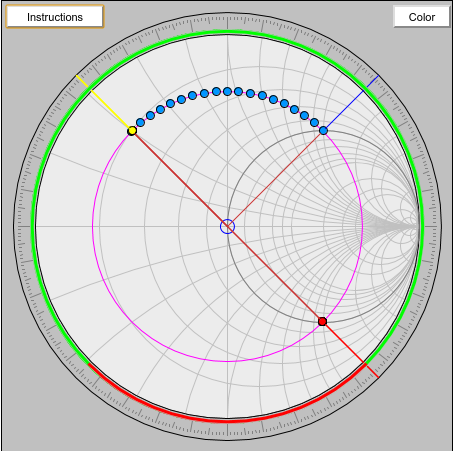
\includegraphics[width=.6\textwidth]{Figures/DValue.png}
            \caption{Smith Chart showing a possible $d$ value}
            \label{fig:1}
          \end{figure}

          As we know that a full circle is equal to $.5\lambda$, we can see that a possible solution, $d$, occurs at:

          $$d=\frac{.5\lambda}{4}=.125(.2)=.025[\si{\meter}]$$

          Thus, we know that we can place the short-circuit stub at $d=.025[\si{\meter}]$ from the load. Next, we need to determine the length of the stub. This is done by finding a value that cancels out the imaginary part. We do this by tracing along towards the axis, following the blue dots:

          \begin{figure}[h!]
            \centering
            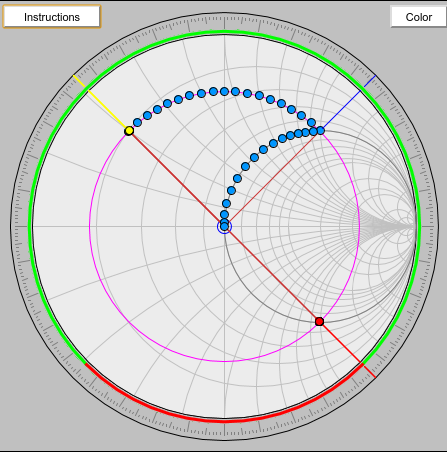
\includegraphics[width=.6\textwidth]{Figures/LValue.png}
            \caption{Smith Chart tracing to an $l$ value}
            \label{fig:2}
          \end{figure}

          As we can see, from Figure \ref{fig:2}, this $d$ value is complemented by a length equal to $l=.0738\lambda$:

          $$l=.0738\lambda=.0738\cdot.2=.01476[\si{\meter}]$$

          As such we obtain a solution with short-circuit stub length $.01476[\si{\meter}]$ located $.025[\si{\meter}]$ from the load. (Note: the steps can be repeated to the second intersection to obtain $d=.25\lambda$ and $l=.42621\lambda$)

      \item 

        Since $\Gamma$ will be equal to zero, now that the circuit is impedance matched, we can simply divide our previous answer by $(.5+|\Gamma|^2)$:

        $$\frac{.3075}{.5}=.615[\si{\watt}]$$

        As expected, this value is greater than the value obtained in Problem 1. This is because, whereas in Problem 1, some of the power was reflected, in Problem 2, all of the power from the incident wave is delivered to the load.

      \item 

        Given the same set up, but with an open stub, we find the $\Gamma$ value to be $|\Gamma|=.781069$. Applying this to the same formula, we get:

        $$\frac{.3075}{.5+(.781069)^2}=.277[\si{\watt}]$$

        Thus, we see that, when incorrectly tuned, the circuit has even worse power delivery to the load, as expected.

    \end{enumerate}

\end{enumerate}

\end{document}

